\documentclass[5pt]{article}
\usepackage[letterpaper, margin=1in]{geometry}
\usepackage{graphicx}
\usepackage{booktabs}
\usepackage{subcaption}

\begin{document}

\title{Assignment 4}
\author{Mukul Sati [msati3@gatech.edu]}
\maketitle

I used the CAFFE framework~\cite{jia2014caffe} for my implementation.

\begin{figure*}[T]
  \centering{}
  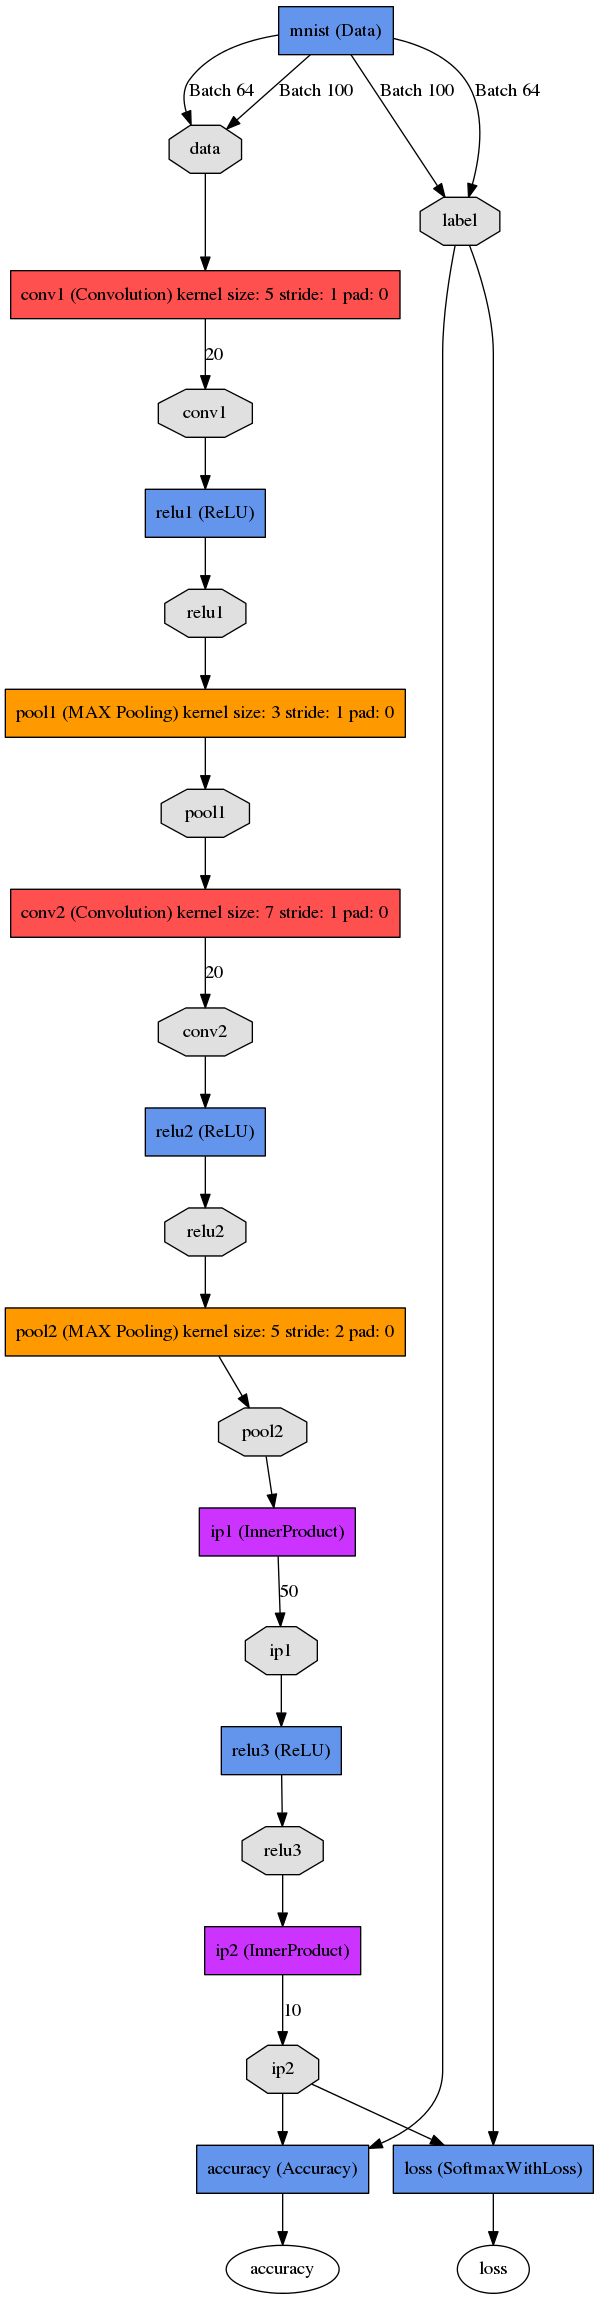
\includegraphics[width=0.9\textwidth]{images/mnist_arch1.png}
  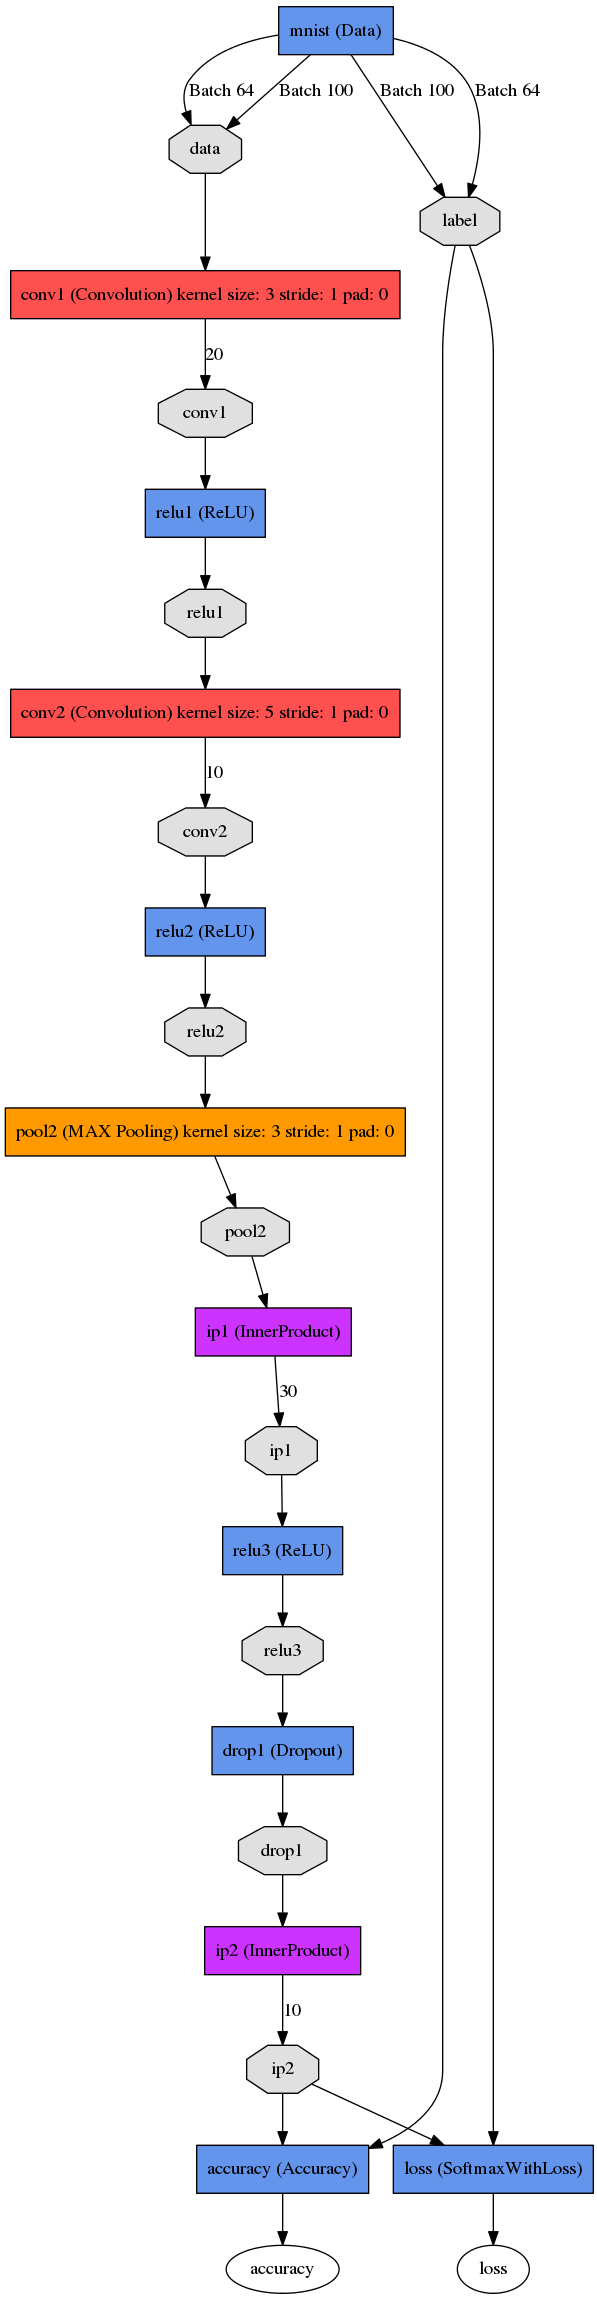
\includegraphics[width=0.9\textwidth]{images/mnist_arch2.png}
  \caption{The two architectures trained for the MNIST dataset.}
\label{fig:mnist_architectures}
\end{figure*}

\section{MNIST Dataset}
I trained two CNN architectures on the MNIST dataset
(Fig.~\ref{fig:mnist_architectures}). I get an accuracy of $XX$ on the first
architecture and $XX$ on the second architecture. The training progress is
shown in Fig.~\ref{fig:mnist_learning}. The kernels learned from the first and
second convolutional layers are visualized in Fig.~\ref{fig:mnist_kernels}.

The following are the gradient descent equations:

\begin{figure}[T]
  \centering{}
  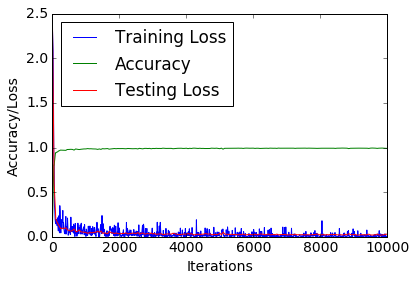
\includegraphics[width=0.4\textwidth]{images/mnist_learning1.png}
  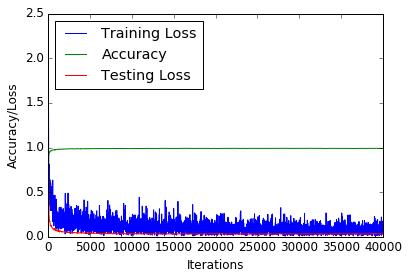
\includegraphics[width=0.4\textwidth]{images/mnist_learning2.png}
  \caption{Training loss and testing loss and accuracy versus iterations for
  the two architectures described above.}
\label{fig:mnist_learning}
\end{figure}

\begin{figure}[T]
  \centering{}
  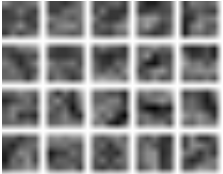
\includegraphics[width=0.4\textwidth]{images/mnist_kernels11.png}
  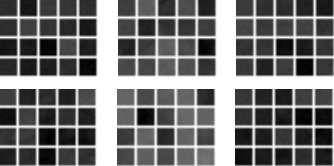
\includegraphics[width=0.4\textwidth]{images/mnist_kernels12.png}
  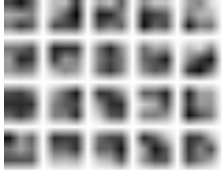
\includegraphics[width=0.4\textwidth]{images/mnist_kernels21.png}
  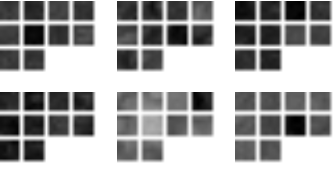
\includegraphics[width=0.4\textwidth]{images/mnist_kernels22.png}
  \caption{The learned filters for the first and second convolutional layers of
  the first and second architectures.}
\label{fig:mnist_kernels}
\end{figure}

\section{Sunset Dataset}
I used the CaffeNet pre-trained network that comes with CAFFE\@. This is pretty
similar to AlexNet, but without the relighting data-augmentation and has a
difference in the order of the pooling and normalization layers. The primary
tweaks I made to CaffeNet are:
\begin{enumerate}
  \item Editing the last fully connected layer for the binary classification
    problem at hand. The initial architecture was for the 1000 class ImageNet
    database.
  \item Lowering the learning rate of the solver, while using a higher
    multiplier for the weights of the modified layer.
\end{enumerate}

Using a very small number of training iterations, I quickly arrive to an
accuracy of about $89\%$ (Fig.~\ref{fig:sunset_vanilla_learning}). After a
longer duration of training, the rate stabilizes at $XX\%$

\begin{figure}[h]
  \centering{}
  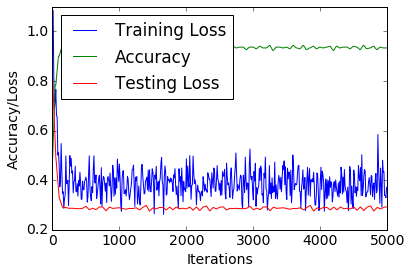
\includegraphics[width=0.8\columnwidth]{images/sunset_vanilla_learning.png}
  \caption{Training loss and testing loss and accuracy versus iterations for
  the vanilla CaffeNet described above.}
\label{fig:sunset_vanilla_learning}
\end{figure}

I use the following schemes for data-augmentation

\medskip
\bibliographystyle{unsrt}
\bibliography{references}

\end{document}
